\chapter{Применение методов} \label{ch3}

% не рекомендуется использовать отдельную section <<введение>> после лета 2020 года
%\section{Введение} \label{ch3:intro}



\section{Модификация сценария ProStack}
\subsection{Описание сценариев}
Для выделения комплексов молекул РНК на исходных данных этой работы применяются два сценария: 

Первый сценарий - \textit{smooth} отвечает за поворот исходного изображения мозга мушки на угол так, чтобы мозг принял обычное горизонтальное положение. Это делается для дальнейшего правильного определения пространственной локализации кластеров генов. Также в этом сценарии происходит обрезка изображения, чтобы в результат попадал только мозг, без пустого окружающего фона.

\begin{figure}[H]
	\centering
	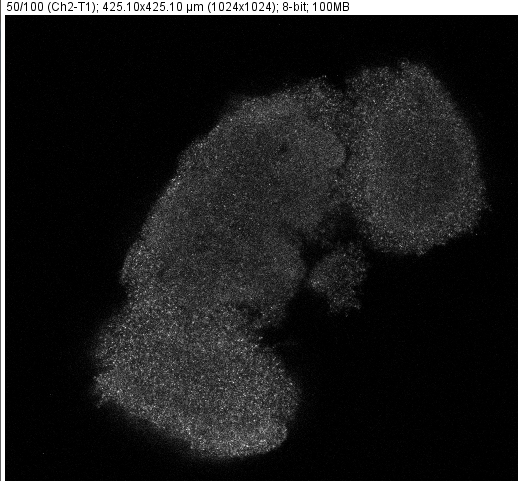
\includegraphics[width=10cm, height=10cm]{smooth_ex_1}
	\caption{Серединный срез 1-го канала изображения мушки дикой породы Sz-139 M5.}
	\label{smooth_ex_1}
\end{figure}

\begin{figure}[H]
	\centering
	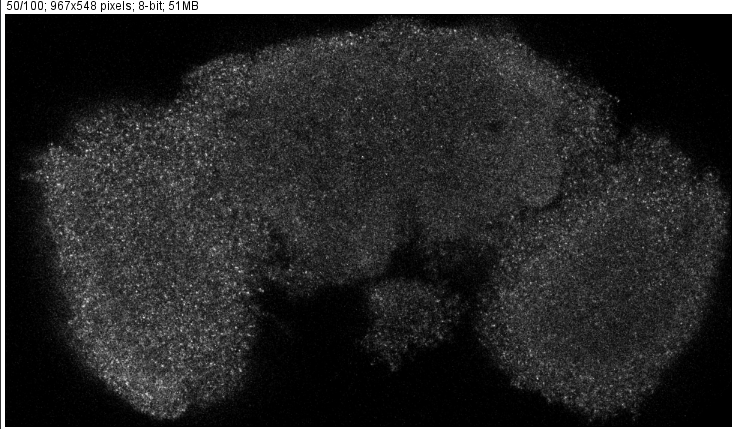
\includegraphics[width=15cm, height=10cm]{smooth_ex_2}
	\caption{Результат обработки сценария \textit{smooth} серединного среза 1-го канала изображения мушки дикой породы Sz-139 M5.}
	\label{smooth_ex_2}
\end{figure}


Второй сценарий - \textit{doots} применяется к результату полученному через предыдущий сценарий (\textit{smooth}). То есть получает на вход повернутый и обрезанный участок мозга мушки. Данный сценарий занимается выделением на изображении комплексов молекул РНК и получением количественных данный экспрессии генов: для каждого найденного участка комплекса молекул РНК сохраняется информация о значении интенсивности пикселей, максимальное значение интенсивности, координаты, номер слоя и др.

Маска комплексов молекул РНК получаемая после применения к изображению на рис. \ref{smooth_ex_2}:

\begin{figure}[H]
	\centering
	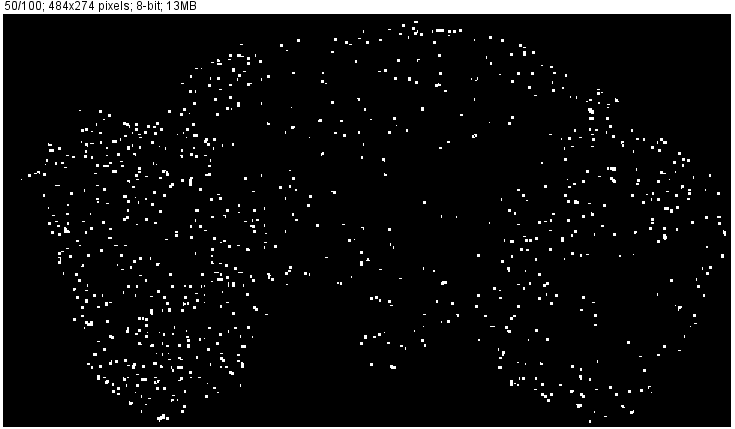
\includegraphics[width=15cm, height=10cm]{doots_ex_1}
	\caption{Результат обработки сценария \textit{doots} серединного среза 1-го канала изображения мушки дикой породы Sz-139 M5.}
	\label{doots_ex_1}
\end{figure}


\subsection{Модификация сценариев}
Для сценария \textit{doots} внесена следующая модификация: 

Для начала рассмотрим участок сценария \textit{doots} в котором происходит удаления фона изображения на рис. \ref{doots_ex_2}. Крайний правый блок (обозначен как \textit{vaff}) удаляет фон, на входе принимает результат работы \textit{smooth} (обозначен как \textit{-sch2-eve}) и результат медианного фильтра по оцененному фону для \textit{-sch2-eve} и находит разность этих входных изображений (из исходного вычитается фон).

\begin{figure}[H]
	\centering
	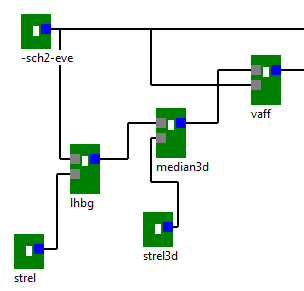
\includegraphics[width=7cm, height=7cm]{doots_ex_2}
	\caption{Участок doots для удаления фона.}
	\label{doots_ex_2}
\end{figure}

Если применять такую же процедуру удаления фона повернутого и обрезанного участка изображения после применения инструмента удаления автофлуоресценции AFid, то результат будет отличен от ожидаемого. Дело в том, что автофлуоресцентные участки заменяются нулевым значениями интенсивности, а значит эти пустые участки будут вносить иной вклад для оценки фона изображения мозга мушки. Результат показан ни рис.\ref{doots_ex_3}.

\begin{figure}[H]
	\centering
	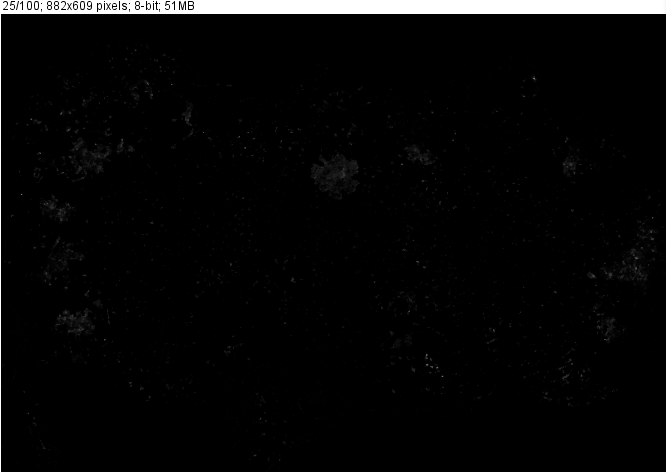
\includegraphics[width=15cm, height=10cm]{doots_ex_3}
	\caption{Результат вычитания фона для 25-го слоя изображения модельной мушки M4 после удаления автофлуоресцентных объектов.}
	\label{doots_ex_3}
\end{figure}

Было принято решение вычитать из обрезанного и повернутого изображения после удаления автофлуоресцентных объектов (обозначение \textit{sch2-eve after AFid}) фон изображения до удаления автофлуоресценции (\textit{-sch2-eve}). Измененная процедура удаления фона показана на рис. 

\begin{figure}[H]
	\centering
	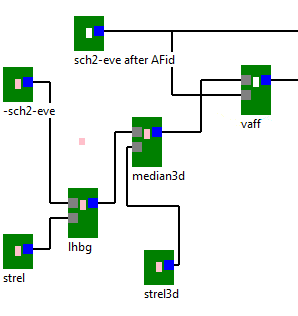
\includegraphics[width=7cm, height=7cm]{doots_ex_5}
	\caption{Модификация участка doots для удаления фона.}
	\label{doots_ex_5}
\end{figure}

Результат такой модификации показан на рисунке \ref{doots_ex_4}. Можно заметить, чтобы остаточный фон для некоторых областей, в отличие от результата на рис. \ref{doots_ex_3} - исчез, а светящиеся точки остались. Значит удаление фона произведено верно.

\begin{figure}[H]
	\centering
	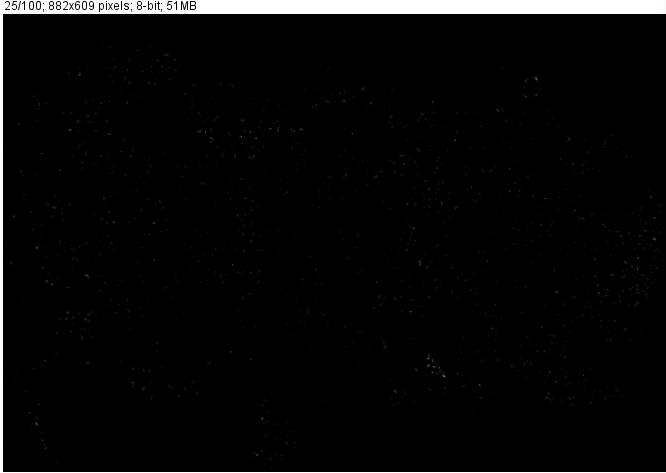
\includegraphics[width=14cm, height=14cm]{doots_ex_4}
	\caption{Результат вычитания фона для 25-го слоя изображения модельной мушки M4 после удаления автофлуоресцентных объектов с учётом модификации.}
	\label{doots_ex_4}
\end{figure}



После модификации сценария \textit{doots}, также потребовались изменения для сценария \textit{smooth}. Дело в том, что размеры результирующего изображения модифицированного сценария \textit{smooth} (обозначали как \textit{sch2-eve after AFid}) и оцененный фон для \textit{-sch2-eve} - результат отработки \textit{smooth} для оригинального изображения (до применения AFid) для вычитания должны иметь одинаковые размеры. После применения инструмента удаления автофлуоресценции, некоторые области мозга удалялись. Это повлияло на результат обрезки сценария \textit{smooth}. То есть в этом случае изображение получалось немного меньше (разница в несколько десятков пикселей). 

Чтобы размеры изображений совпадали, была произведена модификация сценария \textit{smooth} для оригинального изображения. Теперь в сценарии для изображения после удаления автофлуоресцентных объектов сохраняется параметры для обрезания окружающего пустого фона. И эта сохраненная информация используется в сценарии \textit{smooth} для оригинального изображения (до применения AFid). Таким образом, обрезание изображений получается одинаковым и размерности входных данных в блоке удаления фона совпадают.


\section{Алгоритм выделения границ Canny}
Для вычисления количественных данных экспресси генов по изображениям мозга плодовой мушки в сценарий пакета ProStack необходимо добавить алгоритм для выделения границ объектов. В данной работе объекты представляют собой комплексы молекул РНК.

В качестве алгоритма поиска границ был выбран Canny. Это решение связано с низкой воприимчивости к шуму алгоритма и реализацией этого метода в большом количестве пакетов для обработки изображений.

Для применения алгоритма была использована библиотека алгоритмов компьютерного зрения OpenCV. \cite{Booklet}

Для обнаружения границ в исходных данных работы подбирались параметры алгоритма. Так, например, для изображения M7 выделение границ работало хуже с параметрами, которые применялись к остальным изображениям. Для M7 размерность ядра Гауссового размытия было выбрано 4x4 в отличие от 3х3 которое использовалось для остальных изображений.

Параметры алгоритма и шаги выполнения подробно описаны в пункте \ref{canny_algo}. Параметр нижней и верхней границы для утончения границ из шага 4 были выбраны как 30 и 60 соответственно.

На рисунках \ref{canny_in} и \ref{canny_out} представлен пример применения алгоритма обнаружения границ к исходным данным данной работы.

\begin{figure}[H]
	\centering
	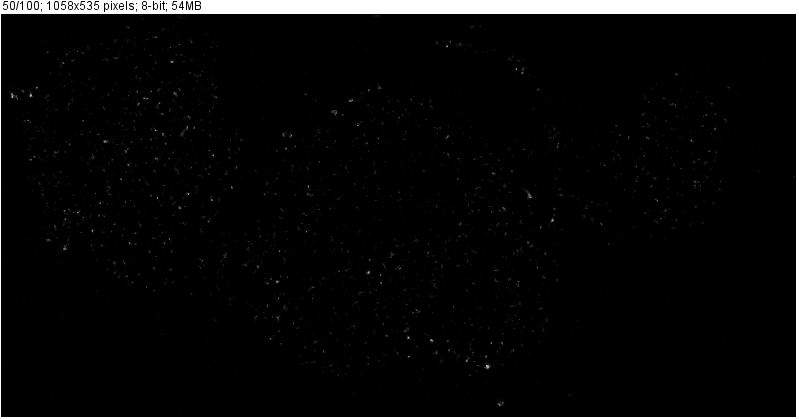
\includegraphics[width=15cm, height=11cm]{canny_in}
	\caption{Серединный срез результата удаления фона изображения M7 мушки дрозофиллы.}
	\label{canny_in}
\end{figure}

\begin{figure}[H]
	\centering
	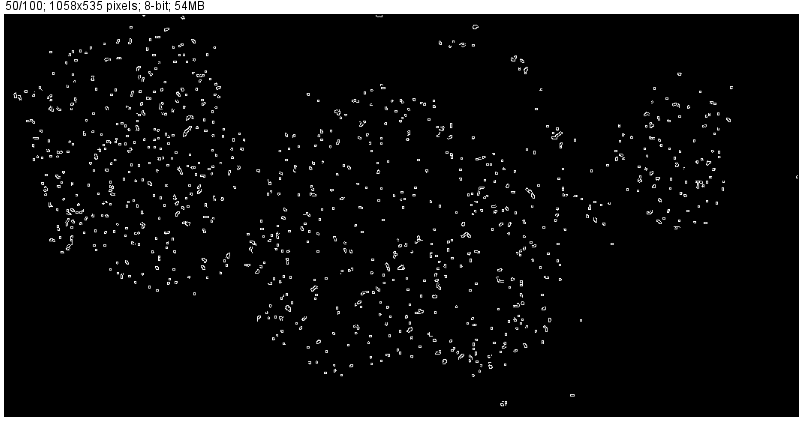
\includegraphics[width=15cm, height=11cm]{canny_out}
	\caption{Серединный срез результата выделения границ объектов после удаления шума изображения M7 мушки дрозофиллы.}
	\label{canny_out}
\end{figure}




\section{Модификация AFid} \label{ch3:sec1}

\subsection{Переписывание на Python}
Алгоритм идентификация автофлуоресцентных объектов AFid был выложен разработчиками в открытом доступе и реализован в пакете Matlab. Из-за некоторых трудностей внедрения приложения написанного на языке требующей лицензии в пакет ProStack, и для доступности использования модификаций для всех пользователей - решено было переписать AFid на языке Python (3.6). %тут ещё надо написать почему питон лучше фиджи и R 

Методы из библиотеки "Image Processing Toolbox" пакета Matlab, которые использовались в AFid  были заменены методами из библиотек skimage, cv2, scipy и sklearn языка Python.


\subsection{Предобработка входных данных}
Одним из требований инструмента AFid было отделение автофлуоресценции от реального сигнала \ref{ch2:subsec-title-abbr}. Но не для всех исходных данных в данной работе данное требование выполнялось. В некоторых изображениях мозга мушки, в одном из каналов наблюдалась почти однородная картина, где комплексы молекул тяжело отделялись, а в другом канале могли быть хорошо отделены.(см. рис \ref{m7_c0c1})
\begin{figure}[H]
	\centering
	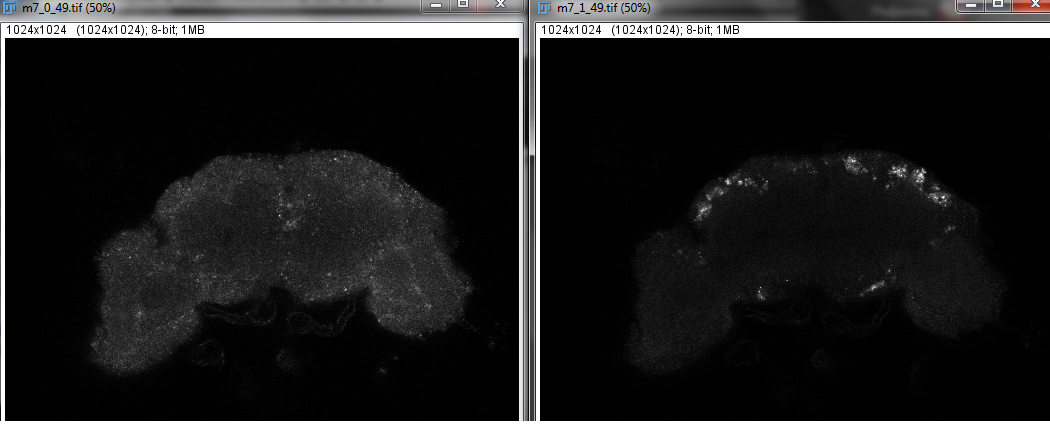
\includegraphics[width=15cm, height=7cm]{m7_c0c1}
	\caption{Серединный срез многослойного трехмерного двухканального изображения R338 M7 мушки дрозофиллы.}
	\label{m7_c0c1}
\end{figure}



В этом случае алгоритм AFid очень неточно генерировал маску пересечения, она получалась слишком однородной, без отделенных сигналов благодаря большому количеству яркого фона в одном из каналов.(см. рис. \ref{m7_mask_no})

\begin{figure}[H]
	\centering
	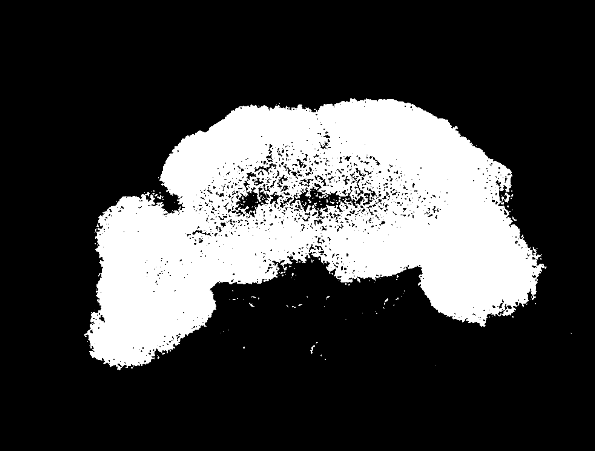
\includegraphics[width=7cm, height=7cm]{m7_mask_no}
	\caption{Маска пересечения до удаление фона.}
	\label{m7_mask_no}
\end{figure}

Было принято решение реазиловать предобработку входных изображений - удалить фон мешающий иентификации областей автофлуоресценции и реальных сигналов.
Удаление фона имеет следующую процедуру:\\
Расчитывается некоторое пороговое значение \textit{d} определемое как\\ $ d = mean value + coeff * std$\\
Тут $ mean value $ -  среднее значение пикслей изображения, $ coeff $ - эмперически подобранный коэффициент равный 0.8, $ std $ - стандартное отклонений значений пикселей изображения.

\begin{figure}[H]
	\centering
	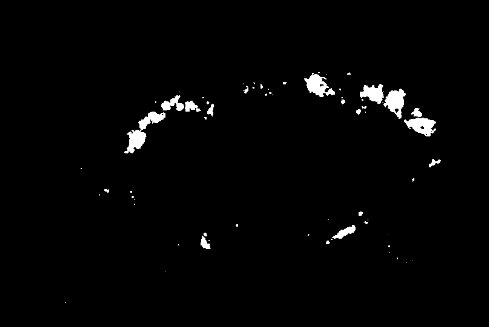
\includegraphics[width=7cm, height=7cm]{m7_mask_yes}
	\caption{Маска пересечения после удаления фона.}
	\label{m7_mask_yes}
\end{figure}

После удаления фона результат выглядит получше, теперь результат умножения масок больше похож на правду, т.к на маске присутствуют объекты которые имеют большую яркость в обеих каналах а не только в первом.(см. рис. \ref{m7_mask_yes})


\subsection{Настройка параметров}
Для применения алгоритма AFid к исходным данным необходимо эмперически подобрать значения параметров, чтобы алгоритм работал как минимум адекватно (не удалял все объекты и находил хотя бы какие-то).

С помощью отладки программы были выявлены некоторые нижние и верхние пороги для параметров применительно к исходным данным:

\begin{enumerate}[1.] \label{afid_params}
	\item \textit{Минимальная и максимальная площадь объектов на изображении}. После нахождения связных областей и свойств для каждого канала изображения, необходимо удалить очень маленькие по площади области. Так, при вычислении межканального коэффициента корреляций Пирсона значений пикселей для каждой области - возникали коэффициенты корреляций равные или очень близкие к 1 или -1, или вовсе появлялись неопределённые значения. Это происходило потому, что области с малой площадью (около 3-4 пикселей) представляли из себя шум, где значение всех пикселей а иногда почти всех - совпадали. Отсюда при вычислении коэффициента корреляций получались указанные выше значения. Также не разумно брать очень большие области, так как иначе при хорошом разделении участков мозга для первой вариации алгоритма с межканальной корреляцией (см.\ref{variations}) в качестве объектов автофлуореценции могут завхватить слишком большие участки мозга. Поэтому нужен верхний порог на площади областей.
	
	Путём сравнения результатов были выбраны следующие пороги: 7 и 50000 - минимальный и максимальный порог для площади связной области соотвественно. 
	
	\item \textit{Значения порогового коэффициента корреляции Пирсона для первой вариации}.
	Изначально стандартным значением для алгоритма было выбрано 0.6, после попытке применить такой параметр к данным этой работы - маски автофлуоресецнтных объектов получались пустыми. Эмперически было подобрано значение 0.3, при меньших значениях появлялись артефакты - громоздкие участи мозга.
	
	
\end{enumerate}




\section{Применение AFid}

Алгоритм AFid применялся к исходным данным описанным в \ref{ch1:sec2} (5 изображений модельной мушки и 4 дикой). Для каждого изображения применялись все три вариации алгоритма (вариации описаны в \ref{variations}) - чтобы сравнить их и выбрать наилучший судя по полученным результатам.
(добавить примеры каждого варианта работы)

После обработки инструментом обнаружения и удаления автофлуоресценции, изображения обрабатывались сценарием пакета Prostack для выделения комплексов молекул РНК и получени количественных данных (интенсивность значений пикселей, координаты выделенных объектов).


\section{Проверка статистической гипотезы}
Инструмент AFid идентифицирует и удаляет автофлуоресцентные объекты. Следовательно, гипотетически, после применения алгоритма паразитное свечение из одного канала в другом должно исчезнуть. Нужно проверить данное предположение. Было решено использовать двухсторонний критерий Вилконсона о наличии следующей гипотезы: медиана смещений среднеквадратичных отклонений значений пикселей выделенных комплексов молекул РНК после применения AFid должна быть отлична от нуля.

Для првоерки критерия, были подготовлены необходимые данные - количественные результаты экспрессии, полученные сценарием ProStack и записанные в файл .csv. Критерий проверялся для пяти изображений модельной мушки и четрырех для дикой породы, по очереди для двух каналов.

Принцип работы критерия Вилконсона в том, что для каждого изображения в двух каналах вычисляются изменения значений среднеквадратичных отклонений значений интенсивностей пикселей с учетом знака. Далее, изменения сортируются без учета знака и каждому значению в отсортированом ряду присваивается
ранг. Подсчитывают суммы рангов для отрицательных изменений и положительных. На основе полученных сумм формируется статистика которую сравнивают с табличным значением квантиля уровня $1 - \frac{\alpha}{2}$ распределения Лапласса. Где $\alpha$ - уровень значимости.

\section{Кластеризация мозга мушки}
Полученные количественные данные сценарием ProStack были кластеризованы методом KMeans, предварительно построены гистограммы значений интенсивности пикселей комплексов молекул РНК: первая гистограмма - учитывала частоту встречаемости пикселей по мере увеличения значения интенсивности, вторая - количество комплексов молекул для каждого слоя изображения. Гистограммы необходимы для удаления вероятного шума,  который в изображениях мозга мушки присутствует в первых либо последних слоях. Также по гистограмме можно выловить шум убирая те выделенные объекты у которых значения интенсивности пикселей очень малое или сильно меньше остальных.\\
(ДОПОЛНИТЬ ПОСЛЕ ВСЕХ РЕЗУЛЬТАТОВ)




\section{Название параграфа} \label{ch3:sec2}

%\FloatBarrier % заставить рисунки и другие подвижные (float) элементы остановиться






%% Вспомогательные команды - Additional commands
%
%\newpage % принудительное начало с новой страницы, использовать только в конце раздела
%\clearpage % осуществляется пакетом <<placeins>> в пределах секций
%\newpage\leavevmode\thispagestyle{empty}\newpage % 100 % начало новой страницы